\begin{document}

\only<article>{
  \thispagestyle{empty}
  \pagecolor{white}\afterpage{\nopagecolor}
  \maketitle
}

\begin{frame}[plain]
 \titlepage
\end{frame}

\frame{
\only<presentation>{
  \frametitle{Inhaltsverzeichnis}
}
\tableofcontents[hideallsubsections]
}

\frame{
\frametitle{Software-Katastrophen}
\begin{block}{Strahlungstod wegen Software-Fehlern}
\begin{itemize}
  \item Bestrahlungsmaschine für Krebspatienten verrechnete sich im Jahr 2000 systematisch bei der Dosierung
  \item Fehler kostete 8 Menschen das Leben, 20 wurden schwer verletzt
  \item Grund: Die Berechnung basierte auf der Reihenfolge, in der Daten eingegeben wurden, was fehlerhafte Eingaben provozierte
\end{itemize}
\end{block}
}

\frame{
\frametitle{Software-Katastrophen}
\begin{block}{NASA Venus-Erkundung}
\begin{itemize}
  \item Venus Mariner 1 geht 1962 unterwegs verloren
  \item Grund: Fehler in FORTRAN-Code, Bindestrich fehlte an einer Stelle im Programmtext
  \item Mit 80 Millionen Dollar Schaden vermutlich der teuerste Bindestrich in der Geschichte der Menschheit
\end{itemize}
\end{block}
}

\frame{
\frametitle{Software-Katastrophen}
\begin{block}{Explosion Ariane 5}
\begin{itemize}
  \item Am 04.06.1996 explodierte Ariane-5-Rakete 40 Sekunden nach dem Start
  \item Verlust ca. 500 Millionen Dollar für Rakete und vier Satelliten
  \item Grund: Überlauf bei Konvertierung von 64-Bit-Wert in 16 Bit signed integer
  \item Übernommene Software stammte von Ariane 4, aber Ariane 5 flog schneller
  \item  Software war für den eigentlichen Flug überflüssig und diente nur den Startvorbereitungen
  \item Video: \href{https://www.youtube.com/watch?v=PK_yguLapgA}{\url{https://www.youtube.com/watch?v=PK_yguLapgA}}
\end{itemize}
\end{block}
}

\frame{
\frametitle{Warum testen wir?}
\begin{block}{}
  \begin{itemize}
    \item Testen ist kosteneffizientes Mittel zur Erkennung von Fehlerzuständen
    \item Testen bietet ein Mittel zur Bewertung der Qualität eines Teilobjektes in verschiedenen Phasen des SDLC (Software Development Life Cycle)
    \item Testen kann auch erforderlich sein, um vertragliche oder gesetzliche Anforderungen zu erfüllen
  \end{itemize}
\end{block}
}

\section{Qualit\"at}

\subsection{Standards}

\frame{
\frametitle{Qualität}
\begin{block}{Definition}
\begin{enumerate}
  \item Grad, in dem ein Satz inhärenter Merkmale eines Objekts Anforderungen erfüllt [ISO 9000]
  \item Grad, in dem eine Komponente oder ein System explizite Bedürfnisse erfüllt [ISO 25010]
  \item Grad, in dem eine Komponente oder ein System implizite Bedürfnisse erfüllt [ISO 25010]
\end{enumerate}
\end{block}
}

\subsection{Grundbegriffe}

\frame{
\frametitle{Verifizierung}
\begin{block}{Definition}
Bestätigung durch Bereitstellung eines objektiven Nachweises, dass festgelegte Anforderungen erfüllt worden sind.
\end{block}
}

\frame{
\frametitle{Validierung}
\begin{block}{Definition}
Bestätigung durch Überprüfung, dass ein Arbeitsergebnis den Bedürfnissen eines Stakeholders entspricht.
\end{block}
}

\frame{
\frametitle{Hauptqualitätsmerkmale von Software}
\begin{center}
\begin{tikzpicture}[scale=.65,transform shape]
  \tikzstyle{level 1 concept}+=[font=\sf, sibling angle=45]
  \path[mindmap,concept color=LightOrange,text=black,every node/.style={concept}]
  node[concept] {Qualität nach ISO 25010} [clockwise from=0]
      child { node[concept] (Functionality) {Funktionale Eignung} }
      child { node[concept] (Reliability) {Zuverlässig\-keit} }
      child { node[concept] (Usability) {Gebrauchs\-tauglichkeit} }
      child { node[concept] (Security) {IT-Sicherheit} }
      child { node[concept] (Maintainability) {Wartbarkeit} }
      child { node[concept] (Efficiency) {Performanz} }
      child { node[concept] (Portability) {Übertrag\-bar\-keit} }
      child { node[concept] (Compatibility) {Kompatibili\-tät} };
\end{tikzpicture}
\end{center}
}

\frame{
\frametitle{Hauptqualitätsmerkmale von Software}
\begin{block}{Funktionale Eignung}
\begin{itemize}
  \item Funktionale Vollständigkeit
  \item Funktionale Richtigkeit
  \item Funktionale Angemessenheit
\end{itemize}
\end{block}
}

\frame{
\frametitle{Hauptqualitätsmerkmale von Software}
\begin{block}{Performanz}
\begin{itemize}
  \item Zeitverhalten 
  \item Ressourcennutzung
  \item Kapazität
\end{itemize}
\end{block}
}

\frame{
\frametitle{Hauptqualitätsmerkmale von Software}
\begin{block}{Kompatibilität}
\begin{itemize}
  \item Koexistenz
  \item Interoperabilität
\end{itemize}
\end{block}
}

\frame{
\frametitle{Hauptqualitätsmerkmale von Software}
\begin{block}{Gebrauchstauglichkeit}
\begin{itemize}
  \item Erkennbare Angemessenheit
  \item Erlernbarkeit
  \item Operabilität
  \item Ästhetik der Benutzungsschnittstelle
  \item Zugänglichkeit
\end{itemize}
\end{block}
}

\frame{
\frametitle{Hauptqualitätsmerkmale von Software}
\begin{block}{Zuverlässigkeit}
\begin{itemize}
  \item Reife
  \item Verfügbarkeit
  \item Fehlertoleranz
  \item Wiederherstellbarkeit
\end{itemize}
\end{block}
}

\frame{
\frametitle{Hauptqualitätsmerkmale von Software}
\begin{block}{IT-Sicherheit}
\begin{itemize}
  \item Vertraulichkeit
  \item Integrität
  \item Nichtabstreitbarkeit
  \item Zurechenbarkeit
  \item Authentizität
\end{itemize}
\end{block}
}

\frame{
\frametitle{Hauptqualitätsmerkmale von Software}
\begin{block}{Wartbarkeit}
\begin{itemize}
  \item Modularität 
  \item Wiederverwendbarkeit
  \item Analysierbarkeit
  \item Modifizierbarkeit
  \item Testbarkeit
\end{itemize}
\end{block}
}

\frame{
\frametitle{Hauptqualitätsmerkmale von Software}
\begin{block}{Übertragbarkeit}
\begin{itemize}
  \item Anpassbarkeit
  \item Installierbarkeit
  \item Austauschbarkeit
\end{itemize}
\end{block}
}

\subsection{Rule of Ten}
\frame{
\frametitle{Rule of Ten}
\begin{block}{Definition}
\begin{itemize}
  \item Im Deutschen als Zehnerregel bekannt
  \item Erfahrungsregel, die besagt, dass die Kosten für die Behebung eines Fehlers mit jedem Schritt im Entwicklungsprozess exponentiell ansteigen
  \item Regel stammt ursprünglich aus der Fertigungstechnik und dem Qualitätsmanagement
  \item Fehlerkosten für einen nicht entdeckten Fehler steigen von Stufe zu Stufe der Wertschöpfung um den Faktor 10
  \item Je früher ein Fehler entdeckt und beseitigt wird, desto kostengünstiger ist dies für die Organisation
\end{itemize}
\end{block}
}

\begin{frame}
\frametitle{Rule of Ten}
\begin{center}
  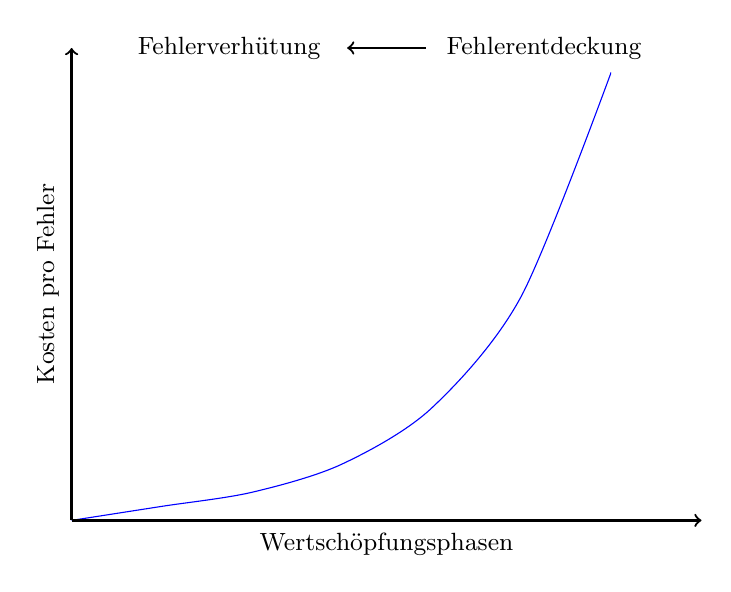
\begin{tikzpicture}[scale=1, every node/.style={scale=1}]
\begin{axis} [
	hide x axis,
	hide y axis,
	axis lines = middle,]
  \addplot[
	smooth,
	thin,
	blue
	] coordinates {
	  (0, 0)
	  (1, .3)
	  (2, .6)
	  (3, 1.2)
	  (4, 2.4)
	  (5, 4.8)
	  (6, 9.6)
	};
\end{axis}

\draw[thick, ->] (0, 0) -- (8, 0);
\draw[thick, ->] (0, 0) -- (0, 6);

\node[rotate=90] at (-.3, 3) {\small Kosten pro Fehler};
\node[] at (4, - .3) {\small Wertsch\"opfungsphasen};
\node[] at (2, 6) {\small Fehlerverh\"utung};
\node[] at (6, 6) {\small Fehlerentdeckung};
\draw[thick, <-] (3.5, 6) -- (4.5, 6);
\end{tikzpicture}
\end{center}
\end{frame}


\section{Testen}

\frame{
\frametitle{Testen}
\begin{block}{Definition}
Prozess, der sämtliche Testaktivitäten umfasst, welche den Zielen dienen
\begin{itemize}
  \item Nachweis der vollständigen Umsetzung der Anforderungen
  \item Nachweis, dass System seinen Zweck erfüllt
  \item Erreichen der festgelegten Qualitätsanforderungen
  \item Aufdecken von etwaigen Fehlerzuständen
\end{itemize}
\end{block}
}

\frame{
\frametitle{Testen}
\setbeamercolor{postit}{fg=black,bg=quoteColor}
\begin{beamercolorbox}[sep=1em,wd=\textwidth]{postit}
  {\large \grqq Program testing can be a very effective way to show the presence of bugs, but is hopelessly inadequate for showing their absence.\grqq}
  \vskip5mm
  \hspace*\fill{\tiny --- Edsger Wybe Dijkstra, The Humble Programmer, ACM Turing Lecture 1972}
\end{beamercolorbox}
}

\subsection{Testziele}

\frame{
\frametitle{Testziele}
\begin{block}{}
  \begin{itemize}
    \item Evaluieren von Arbeitsergebnissen wie Anforderungen, User Storys, Entwürfe und Code
    \item Auslösen von Fehlerwirkungen und Finden von Fehlerzuständen
    \item Sicherstellen der erforderlichen Überdeckung eines Testobjekts
    \item Verringern des Risikos einer unzureichenden Softwarequalität
    \item Verifizieren, ob ein Testobjekt den vertraglichen, rechtlichen und regulatorischen Anforderungen entspricht
  \end{itemize}
\end{block}
}

\frame{
\frametitle{Testziele}
\begin{block}{}
  \begin{itemize}
    \item Bereitstellen von Informationen für die Stakeholder, damit diese fundierten Entscheidungen treffen können (z.B. Freigabeentscheidung eines Releases)
    \item Aufbauen von Vertrauen in die Qualität des Testobjekts
    \item Validieren, ob das Testobjekt vollständig ist und aus Sicht der Stakeholder wie erwartet funktioniert
  \end{itemize}
\end{block}
}

\subsection{Testprozess}

\frame{
\frametitle{Fundamentaler Testprozess nach ISTQB}
\begin{center}
\begin{tikzpicture}
\node (Beginn)       at (0,3)  [fill=LightOrange,minimum height=0.75em,text width=1cm,ellipse, text centered] {Beginn};
\node (Planung)      at (0,2)  [rectangle, fill=LightOrange,   text width=6cm, minimum height=1em, text centered, rounded corners=8pt] {Planung und Steuerung};
\node (Analyse)      at (0,1)  [rectangle, fill=LightOrange,   text width=6cm, minimum height=1em, text centered, rounded corners=8pt] {Analyse und Design};
\node (Realisierung) at (0,0)  [rectangle, fill=LightOrange,   text width=6cm, minimum height=1em, text centered, rounded corners=8pt] {Realisierung und Durchf\"uhrung};
\node (Auswertung)   at (0,-1) [rectangle, fill=LightOrange,   text width=6cm, minimum height=1em, text centered, rounded corners=8pt] {Auswertung und Bericht};
\node (Abschluss)    at (0,-2) [rectangle, fill=LightOrange,   text width=6cm, minimum height=1em, text centered, rounded corners=8pt] {Abschluss};
\node (Ende)         at (0,-3) [fill=LightOrange,minimum height=0.75em,text width=1cm,ellipse, text centered] {Ende};
\draw[->, very thick](Beginn) to node[right]{} (Planung);
\draw[->, very thick](Planung) to node[right]{} (Analyse);
\draw[->, very thick](Analyse) to node[right]{} (Realisierung);
\draw[->, very thick](Realisierung) to node[right]{} (Auswertung);
\draw[->, very thick](Auswertung) to node[right]{} (Abschluss);
\draw[->, very thick](Abschluss) to node[right]{} (Ende);
\draw[<-, very thick](Analyse) to[bend left=90] node[right]{} (Auswertung);
\draw[<-, very thick](Realisierung) to[bend left=90] node[right]{} (Auswertung);
\draw[->, very thick](Abschluss) to[bend left=90] node[right]{} (Planung);
\draw[->, very thick](Abschluss) to[bend left=90] node[right]{} (Analyse);
\end{tikzpicture}
\end{center}
}

\subsection{Prinzipien}
\frame{
\frametitle{Allgemeine Prinzipien des Softwaretestens}
\begin{itemize}
	\item Testen zeigt Anwesenheit von Fehlern, nicht die Abwesenheit von Fehlerzuständen
	\item Vollständiges Testen ist unmöglich
	\item Frühes Testen spart Geld und Zeit
	\item Fehlerzustände treten gehäuft auf
	\item Tests nutzen sich ab (Testresistenz)
	\item Testen ist kontextabhängig
	\item Trugschluss: Keine Fehler bedeuten ein brauchbares System
\end{itemize}
}

\subsection{Fehlerbegriff}

\frame{
\frametitle{Fehlerbegriff}
\begin{block}{}
  \begin{itemize}
    \item Menschen begehen Fehlhandlungen (Irrtümer, errors)
    \item Fehlhandlungen führen zu Fehlerzuständen (Defekten, bugs, defects, faults)
    \item Fehlerwirkungen (failures) können durch Fehlerzuständen ausgelöst werden
    \item Fehlerwirkungen können auch durch Umweltbedingungen verursacht werden
  \end{itemize}
\end{block}
}

\frame{
\frametitle{Fehlerbegriff}
\begin{center}
\begin{tikzpicture}
\node (Fehlhandlung) at (0,0)  [rectangle, fill=LightOrange,   text width=6cm, minimum height=1em, text centered, rounded corners=8pt] {Fehlhandlung (error)};
\node (Fehlerzustand) at (0,-1.5)  [rectangle, fill=LightOrange,   text width=6cm, minimum height=1em, text centered, rounded corners=8pt] {Fehlerzustand (bug, defect, fault)};
\node (Fehlerwirkung) at (0,-3)  [rectangle, fill=LightOrange,   text width=6cm, minimum height=1em, text centered, rounded corners=8pt] {Fehlerwirkung (failure)};
\node (Schaden) at (0,-4.5)  [rectangle, fill=LightOrange,   text width=6cm, minimum height=1em, text centered, rounded corners=8pt] {Schaden};
\draw[->, very thick](Fehlhandlung) to node{} (Fehlerzustand);
\draw[->, very thick](Fehlerzustand) to node{} (Fehlerwirkung);
\draw[->, very thick](Fehlerwirkung) to node{} (Schaden);
\end{tikzpicture}
\end{center}
}

\frame{
\frametitle{Beispiel: Fehlerbegriff}
\begin{center}
\begin{tikzpicture}
\node (Fehlhandlung) at (0,0)  [rectangle, fill=LightOrange,   text width=3cm, minimum height=1em, text centered, rounded corners=8pt] {Fehlhandlung};
\node at (5.75,0) [text width=7cm,fill=ivory, rounded corners=8pt] {Nutzer teilt 5 durch 0};
\node (Fehlerzustand) at (0,-1.75)  [rectangle, fill=LightOrange,   text width=3cm, minimum height=4em, text centered, rounded corners=8pt] {Fehlerzustand};
\node at (5.75,-1.75) [text width=7cm,fill=ivory, rounded corners=8pt] {int dividend = 5;\\int divisor = 0;\\double result = dividend / divisor;};
\node (Fehlerwirkung) at (0,-3.5)  [rectangle, fill=LightOrange,   text width=3cm, minimum height=1em, text centered, rounded corners=8pt] {Fehlerwirkung};
\node at (5.75,-3.5) [text width=7cm,fill=ivory, rounded corners=8pt] {java.lang.ArithmeticException: / by zero};
\node (Schaden) at (0,-4.75)  [rectangle, fill=LightOrange,   text width=3cm, minimum height=1em, text centered, rounded corners=8pt] {Schaden};
\node at (5.75,-4.75) [text width=7cm,fill=ivory, rounded corners=8pt] {Kunde fordert Nachbesserung};
\draw[->, very thick](Fehlhandlung) to node{} (Fehlerzustand);
\draw[->, very thick](Fehlerzustand) to node{} (Fehlerwirkung);
\draw[->, very thick](Fehlerwirkung) to node{} (Schaden);
\end{tikzpicture}
\end{center}
}

\frame{
\frametitle{Fehlerkultur}
\begin{itemize}
  \item Fehler eingestehen
  \item Fehler nicht sanktionieren
  \item Aus Fehlern lernen
  \item Fehler sollen nicht blockieren
  \item Fehler finden ist positiv
  \item Fehler vom Verursacher beheben lassen
  \item Fehler kommunizieren
\end{itemize}
}

\subsection{Debugging}
\frame{
\frametitle{Debugging}
\begin{block}{Definition}
\begin{itemize}
	\item Prozess der Aufdeckung, Analyse und Entfernung der Ursache von Fehlerwirkungen in einer Komponente oder einem Fehler
	\item Typischer Debugging-Prozess:
	\begin{itemize}
		\item Reproduzieren einer Fehlerwirkung
		\item Diagnose (Befund einer Grundursache)
		\item Behebung der Ursache
	\end{itemize}
	\item Debugging erfolgt in der Regel durch den Entwickler
\end{itemize}
\end{block}
}

\subsection{Testarten}

\frame{
\frametitle{Testart}
\begin{block}{Definition}
Eine Gruppe von Testaktivitäten basierend auf bestimmten Testzielen mit dem Zweck, eine Komponente oder ein System auf spezifische Merkmale zu prüfen.
\end{block}
}

\frame{
\frametitle{Testarten}
\begin{block}{Testarten}
\begin{itemize}
\item Funktionaler Test
\item Nicht-funktionaler Test
\item Black-Box-Test
\item White-Box-Test
\end{itemize}
\end{block}
}

\frame{
\frametitle{Testarten}
\begin{block}{Funktionaler Test}
Testen, welches durchgeführt wird, um die Erfüllung der funktionalen Anforderungen durch eine Komponente oder ein System zu bewerten.
\end{block}
}

\frame{
\frametitle{Testarten}
\begin{block}{Nicht-funktionaler Test}
Testen, welches durchgeführt wird, um die Erfüllung der nicht-funktionalen Anforderungen durch eine Komponente oder ein System zu bewerten.
\end{block}
}

\frame{
\frametitle{Black-Box-Test}
\begin{block}{Definition}
Testen auf der Grundlage einer Analyse der Spezifikation der Komponente oder des Systems.
\end{block}
}

\frame{
\frametitle{White-Box-Test}
\begin{block}{Definition}
Ein Test, der auf der Analyse der internen Struktur einer Komponente oder eines Systems basiert.
\end{block}
}

\subsection{Testverfahren}

\frame{
\frametitle{Testbedingung}
\begin{block}{Definition}
Ein testbarer Aspekt einer Komponente oder eines Systems, der als Grundlage für das Testen identifiziert wurde.
\end{block}
}

\frame{
\frametitle{Testdaten}
\begin{block}{Definition}
Für die Testdurchführung benötigte Daten.
\end{block}
}

\frame{
\frametitle{Testverfahren}
\begin{block}{Definition}
Eine Vorgehensweise zum Definieren von Testbedingungen, Entwerfen von Testfällen und Spezifizieren von Testdaten.
\end{block}
}

\frame{
\frametitle{Testverfahren}
\begin{center}
\begin{tikzpicture}
\node at (4.5,3.5) [rectangle, fill=LightOrange, text width=10.6cm, minimum height=4em, text centered, rounded corners=8pt] {Testverfahren};

\node at (2.2,1.75) [rectangle, fill=LightOrange, text width=6.1cm, minimum height=4em, text centered, rounded corners=8pt] {Dynamische Testverfahren};
\node at (7.85,1.75) [rectangle, fill=LightOrange, text width=3.9cm, minimum height=4em, text centered, rounded corners=8pt] {Statische Testverfahren};

\node at (0,0) [rectangle, fill=LightOrange, text width=1.75cm, minimum height=4em, text centered, rounded corners=8pt] {Black-Box};
\node at (2.2,0) [rectangle, fill=LightOrange, text width=1.75cm, minimum height=4em, text centered, rounded corners=8pt] {White-Box};
\node at (4.4,0) [rectangle, fill=LightOrange, text width=1.75cm, minimum height=4em, text centered, rounded corners=8pt] {erfahrungs\-basiert};
\node at (6.8,0) [rectangle, fill=LightOrange, text width=1.75cm, minimum height=4em, text centered, rounded corners=8pt] {Reviews};
\node at (9,0) [rectangle, fill=LightOrange, text width=1.75cm, minimum height=4em, text centered, rounded corners=8pt] {statische Analysen};
\end{tikzpicture}
\end{center}
}

\section{Dynamische Testverfahren}
\subsection{Black-Box-Testverfahren}
\frame{
\frametitle{Black-Box-Testverfahren}
\begin{block}{Definition}
Ein Testverfahren, das auf einer Analyse der Spezifikation einer Komponente oder eines Systems basiert.
\end{block}
}

\frame{
\frametitle{Black-Box-Testverfahren}
\begin{itemize}
  \item Äquivalenzklassenbildung
  \item Grenzwertanalyse
  \item Entscheidungstabellen
  \item Zustandsbasierte Verfahren
  \item Anwendungsfallbasierte Verfahren
\end{itemize}
}

\frame{
\frametitle{Äquivalenzklasse}
\begin{block}{Definition}
Eine Teilmenge des Wertebereichs einer Variablen innerhalb einer Komponente oder eines Systems, für die aufgrund der Spezifikation erwartet wird, dass alle Werte gleichartig behandelt werden.
\end{block}
}

\frame{
\frametitle{Beispiel: Äquivalenzklassenbildung}
\begin{block}{Anforderungen}
\begin{itemize}
  \item Überschreitet ein Verkehrsteilnehmer die Geschwindigkeit ($v$) um mehr als 3 km/h bis einschließlich 10 km/h, beträgt die Strafe 20 Euro.
  \item Überschreitet ein Verkehrsteilnehmer die Geschwindigkeit ($v$) um mehr als 10 km/h bis einschließlich 20 km/h, beträgt die Strafe 50 Euro.
  \item Überschreitet ein Verkehrsteilnehmer die Geschwindigkeit ($v$) um mehr als 20 km/h, beträgt die Strafe 100 Euro.
  \item Die Geschwindigkeitsüberschreitung wird als ganze Zahl angegeben.
\end{itemize}
\end{block}
}

\frame{
\frametitle{Beispiel: Äquivalenzklassenbildung}
\begin{itemize}
  \item 3 gültige Äquivalenzklassen
  \begin{itemize}
    \item Zulässige Vertreter der drei Äquivalenzklassen, z.\,B. 6, 13 und 41.
  \end{itemize}
  \item 1 ungültige Äquivalenzklasse
  \begin{itemize}
    \item Zulässiger Vertreter der Äquivalenzklasse, z.\,B. 2.
  \end{itemize}
\end{itemize}
\begin{center}
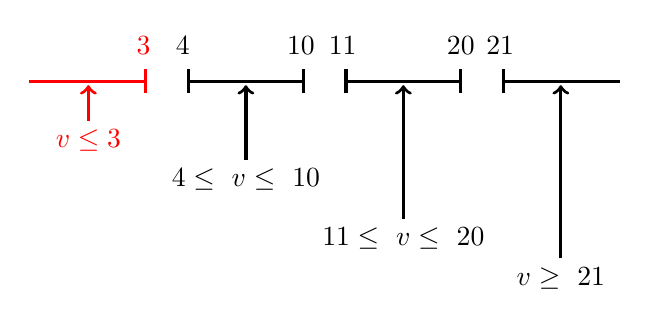
\begin{tikzpicture}
\node at (.95, .45) [color=red]{3};
\draw[-|, very thick, color=red](-.5,0) -- (1,0);
\node at (1.45, .45) {4};
\node at (2.95, .45) {10};
\draw[|-|, very thick](1.5,0) -- (3,0);
\node at (3.48, .45) {11};
\node at (4.98, .45) {20};
\draw[|-|, very thick](3.5,0) -- (5,0);
\draw[->, very thick, color=red](.25,-.5) -- (0.25,-.05);
\node at (.25, -.75) [color=red]{$v \leq 3$};
\draw[->, very thick](2.25,-1) -- (2.25,-.05);
\node at (2.25, -1.25) {$4 \leq\ v \leq\ 10$};
\draw[->, very thick](4.25,-1.75) -- (4.25,-.05);
\node at (4.25, -2) {$11 \leq\ v \leq\ 20$};
\node at (5.48, .45) {21};
\draw[|-, very thick](5.5,0) -- (7,0);
\draw[->, very thick](6.25,-2.25) -- (6.25,-.05);
\node at (6.25, -2.5) {$ v \geq\ 21$};
\end{tikzpicture}
\end{center}
}

\frame{
\frametitle{Grenzwertanalyse}
\begin{block}{Definition}
Ein Black-Box-Testverfahren, bei dem die Testfälle unter Nutzung von Grenzwerten entworfen werden.
\end{block}
}

\frame{
\frametitle{Beispiel: Grenzwertanalyse}
\begin{itemize}
  \item 3 km/h (ungültige Eingabe)
  \item 4 km/h (gültige Eingabe)
  \item 10 km/h (gültige Eingabe)
  \item 11 km/h (gültige Eingabe)
  \item 20 km/h (gültige Eingabe)
  \item 21 km/h (gültige Eingabe)
\end{itemize}
\begin{center}
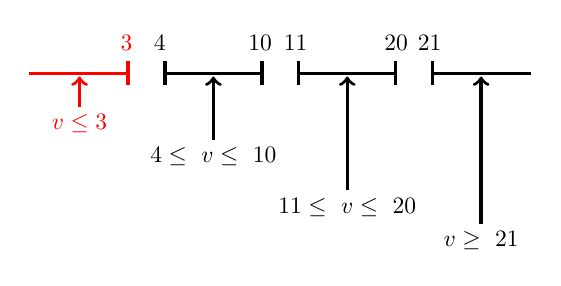
\begin{tikzpicture}[scale=.85,transform shape]
\node at (.95, .45) [color=red]{3};
\draw[-|, very thick, color=red](-.5,0) -- (1,0);
\node at (1.45, .45) {4};
\node at (2.95, .45) {10};
\draw[|-|, very thick](1.5,0) -- (3,0);
\node at (3.48, .45) {11};
\node at (4.98, .45) {20};
\draw[|-|, very thick](3.5,0) -- (5,0);
\draw[->, very thick, color=red](.25,-.5) -- (0.25,-.05);
\node at (.25, -.75) [color=red]{$v \leq 3$};
\draw[->, very thick](2.25,-1) -- (2.25,-.05);
\node at (2.25, -1.25) {$4 \leq\ v \leq\ 10$};
\draw[->, very thick](4.25,-1.75) -- (4.25,-.05);
\node at (4.25, -2) {$11 \leq\ v \leq\ 20$};
\node at (5.48, .45) {21};
\draw[|-, very thick](5.5,0) -- (7,0);
\draw[->, very thick](6.25,-2.25) -- (6.25,-.05);
\node at (6.25, -2.5) {$ v \geq\ 21$};
\end{tikzpicture}
\end{center}
}

\frame{
\frametitle{Entscheidungstabellentest}
\begin{block}{Definition}
Ein Black-Box-Testverfahren, bei dem Testfälle im Hinblick auf die Ausführung von Kombinationen der Bedingungen und aus ihnen resultierender Aktionen einer Entscheidungstabelle entworfen werden.
\end{block}
}

\frame{
\frametitle{Beispiel: Entscheidungstabellentest}
\begin{block}{Vollständige Entscheidungstabelle}
\begin{tabular}{|p{5cm}|l|l|l|l|l|l|l|l|}
\hline
\rowcolor{ivory}
\textbf{Testfall-ID} & \textbf{1} & \textbf{2} & \textbf{3} & \textbf{4} & \textbf{5} & \textbf{6} & \textbf{7} & \textbf{8} \\\hline
\rowcolor{ivory}
\multicolumn{9}{|l|}{\textbf{Bedingungen}} \\ \hline
1 Lieferfähig?               & T & T & T & T & F & F & F & F\\ \hline
2 Angaben vollständig?       & T & T & F & F & T & T & F & F\\ \hline
3 Bonität in Ordnung?        & T & F & T & F & T & F & T & F\\ \hline
\rowcolor{ivory}
\multicolumn{9}{|l|}{\textbf{Aktionen}} \\ \hline
A Lieferung mit Rechnung     & X &   &   &   &   &   &   & \\ \hline
B Lieferung als Nachnahme    &   & X &   &   &   &   &   & \\ \hline
C Angaben vervollständigen   &   &   & X & X &   &   &   & \\ \hline
D Mitteilen: nicht lieferbar &   &   &   &   & X & X & X & X\\ \hline
\end{tabular}
\end{block}
}

\frame{
\frametitle{Beispiel: Entscheidungstabellentest}
\begin{block}{Reduzierte Entscheidungstabelle}
\begin{tabular}{|p{5cm}|l|l|l|l|}
\hline
\rowcolor{ivory}
\textbf{Testfall-ID} & \textbf{1} & \textbf{2} & \textbf{4'} & \textbf{5'} \\\hline
\rowcolor{ivory}
\multicolumn{5}{|l|}{\textbf{Bedingungen}} \\ \hline
1 Lieferfähig?               & T & T & T & F \\ \hline
2 Angaben vollständig?       & T & T & F & - \\ \hline
3 Bonität in Ordnung?        & T & F & - & - \\ \hline
\rowcolor{ivory}
\multicolumn{5}{|l|}{\textbf{Aktionen}} \\ \hline
A Lieferung mit Rechnung     & X &   &   &   \\ \hline
B Lieferung als Nachnahme    &   & X &   &   \\ \hline
C Angaben vervollständigen   &   &   & X &   \\ \hline
D Mitteilen: nicht lieferbar &   &   &   & X \\ \hline
\end{tabular}
\end{block}
}

\frame{
\frametitle{Zustandsübergangstest}
\begin{block}{Definition}
Ein Black-Box-Testverfahren, bei dem Testfälle entworfen werden, um Elemente eines Zustandsübergangsmodells auszuführen.
\end{block}
}

\frame{
\frametitle{Beispiel: Zustandsübergangstest}
\begin{center}
\begin{tikzpicture}[scale=.95,transform shape]
\node (S1) at (0,2) [rectangle, fill=LightOrange, text width=4cm, minimum height=1em, text centered, rounded corners=8pt] {TV Off (S1)};

\node (S2) at (0,0) [rectangle, fill=LightOrange, text width=4cm, minimum height=1em, text centered, rounded corners=8pt] {TV Stand By (S2)};

\node (S3) at (7.5,1) [rectangle, fill=LightOrange, text width=3cm, minimum height=3cm, text centered, rounded corners=8pt] {TV Play (S3)};

\draw[->, very thick](5.75,2) -- (2.25, 2);
\node at (4, 2.3) {Power Off};

\draw[<-, very thick](5.75,.25) -- (2.25, .25);
\node at (4, .5) {RC On};

\draw[->, very thick](5.75, -.25) -- (2.25, -.25);
\node at (4, -.55) {RC Off};

\draw[->, very thick](.5, .4) -- (.5, 1.65);
\node at (1.5, 1) {Power Off};

\draw[<-, very thick](-.5, .4) -- (-.5, 1.65);
\node at (-1.5, 1) {Power On};
\end{tikzpicture}
\end{center}
\begin{tabular}{|l|l|l|l|l|l|}
\hline
\rowcolor{ivory}
\textbf{Testfall} & \textbf{1} & \textbf{2} & \textbf{3} & \textbf{4} & \textbf{5}\\ \hline
Startzustand & S1 & S2 & S2 & S3 & S3\\ \hline
Eingabe & Power On & Power Off & RC On & RC Off & Power Off\\ \hline
Endzustand & S2 & S1 & S3 & S2 & S1\\ \hline
\end{tabular}
}

\frame{
\frametitle{Anwendungsfall-Test}
\begin{block}{Definition}
Ein Black-Box-Testverfahren, bei dem Testfälle entworfen werden im Hinblick auf die Ausführung verschiedener Verhalten eines Anwendungsfalls.
\end{block}
}

\subsection{White-Box-Testverfahren}
\frame{
\frametitle{White-Box-Testverfahren}
\begin{block}{Definition}
Ein Testverfahren, das nur auf der inneren Struktur einer Komponente oder eines Systems basiert.
\end{block}
}

\frame{
\frametitle{White-Box-Testverfahren}
\begin{itemize}
	\item Anweisungsüberdeckung
	\item Entscheidungsüberdeckung
	\item Pfadüberdeckung
	\item Einfache und mehrfache Bedingungsüberdeckung
\end{itemize}
}

\frame{
\frametitle{Anweisungsüberdeckung}
\begin{block}{Definition}
\begin{itemize}
  \item Jede Anweisung wird mindestens einmal getestet
  \item Deckt nicht erreichbare Anweisungen (dead code) im Quelltext auf
  \item Bei Verzweigungen (z.\,B. Schleifen, Bedingungen) werden Datenabhängigkeiten nicht beachtet
\end{itemize}
\end{block}
}

\begin{frame}[fragile]
\frametitle{Beispiel: Anweisungsüberdeckung}
\begin{block}{}
\begin{lstlisting}[language=Java]
int calcSum(int value) {
  int sum = 0;
  int i = 0;
  while(i < value) {
    sum += ++i;
  }
  return sum;
}
\end{lstlisting}
Ein Testfall ist notwendig, um alle Anweisungen abzudecken
\begin{itemize}
  \item Testfall 1: \lstinline{value = 3}
\end{itemize}
\end{block}
\end{frame}

\frame{
\frametitle{Entscheidungsüberdeckung}
\begin{block}{Definition}
\begin{itemize}
  \item Durchläuft alle Zweige des Quellcodes
  \item 100\% Entscheidungsüberdeckung schließt 100\% der Anweisungen ein
\end{itemize}
\end{block}
}

\begin{frame}[fragile]
\frametitle{Beispiel: Entscheidungsüberdeckung}
\begin{block}{}
\begin{lstlisting}[language=Java]
int calcSum(int value) {
  int sum = 0;
  int i = 0;
  while(i < value) {
    sum += ++i;
  }
  return sum;
}
\end{lstlisting}
Zwei Testfälle sind notwendig, um alle Entscheidungen abzudecken
\begin{itemize}
  \item Testfall 1: \lstinline{value = 0}
  \item Testfall 2: \lstinline{value = 3}
\end{itemize}
\end{block}
\end{frame}

\frame{
\frametitle{Pfadüberdeckung}
\begin{block}{Definition}
Testmethode, welche die Ausführung aller möglichen Pfade vom Start- zum Endknoten des Testobjektes erfordert
\end{block}
}

\frame{
\frametitle{Beispiel: Pfadüberdeckung}
\tikzstyle{state} = [circle, text centered, draw=black, fill=LightOrange]
\tikzstyle{arrow} = [->,>=stealth]
\begin{center}
\begin{tikzpicture}[scale=1,transform shape]
\node (start) [circle,fill=black] at (-1.25,0) {};
\node (S1) [state] at (0,0) {S1};
\node (S2) [state] at (1.25,1.25) {S2};
\node (S3) [state] at (2.25,0) {S3};
\node (S4) [state] at (4,0) {S4};
\node (S5) [state] at (5,1.25) {S5};
\node (S6) [state] at (6.25,0) {S6};
\node (stop) [circle,draw=black] at (7.5,0) {};
\fill (7.5,0) circle(0.1);
\draw [arrow](-1.25,0) -- node[anchor=north]{a} (S1);
\draw [arrow](S1) -- node[anchor=east]{b} (S2);
\draw [arrow](S1) -- node[anchor=north]{d} (S3);
\draw [arrow](S2) -- node[anchor=west]{c} (S3);
\draw [arrow](S3) -- node[anchor=north]{e} (S4);
\draw [arrow](S4) -- node[anchor=east]{f} (S5);
\draw [arrow](S4) -- node[anchor=north]{h} (S6);
\draw [arrow](S5) -- node[anchor=west]{g} (S6);
\draw [arrow](S6) -- node[anchor=south]{i} (stop);
\end{tikzpicture}
\end{center}
4 Testfälle für 100\%-ige Pfadüberdeckung:
\begin{itemize}
  \item abcefgi
  \item abcehi
  \item adefgi
  \item adehi
\end{itemize}
}

\frame{
\frametitle{Einfache und mehrfache Bedingungsüberdeckung}
\begin{block}{Definitionen}
\begin{itemize}
  \item \textbf{Einfache Bedingungsüberdeckung}:\newline Jede atomare Bedingung einer Entscheidung muss einmal mit \lstinline{true} und einmal mit \lstinline{false} getestet werden.
  \item \textbf{Mehrfache Bedingungsüberdeckung}:\newline Dieser Test betrachtet alle atomaren Bedingungen einer Bedingung. Wenn $n$ atomare Bedingungen in der Bedingung stehen, dann werden $2^n$ Kombinationen gebildet. 
\end{itemize}
\end{block}
}

\begin{frame}[fragile]
\frametitle{Beispiel: Einfache Bedingungsüberdeckung}
\begin{block}{}
\begin{lstlisting}[language=Java]
void dummy(boolean a, boolean b) {
  if (a || b) {
    System.out.println("then");
  }
}
\end{lstlisting}

Zwei Testfälle sind notwendig, da jede Bedingung einmal \lstinline{true} und einmal \lstinline{false} sein muss:
\begin{itemize}
  \item Testfall 1: \lstinline{a=false} und \lstinline{b=false}
  \item Testfall 2: \lstinline{a=true} und \lstinline{b=true}
\end{itemize}
\end{block}
\end{frame}

\begin{frame}[fragile]
\frametitle{Beispiel: Mehrfache Bedingungsüberdeckung}
\begin{block}{}
\begin{lstlisting}[language=Java]
void dummy(boolean a, boolean b) {
  if (a || b) {
    System.out.println("then");
  }
}
\end{lstlisting}

Vier Testfälle sind notwendig:
\begin{itemize}
  \item Testfall 1: \lstinline{a=false} und \lstinline{b=false}
  \item Testfall 2: \lstinline{a=true} und \lstinline{b=true}
  \item Testfall 3: \lstinline{a=false} und \lstinline{b=true}
  \item Testfall 4: \lstinline{a=true} und \lstinline{b=false}
\end{itemize}
\end{block}
\end{frame}

\frame{
\frametitle{Vergleich Black- und White-Box-Testverfahrens}
\begin{itemize}
  \item Vorteile von Black-Box-Tests gegenüber White-Box-Tests 
  \begin{itemize}
    \item Bessere Verifikation des Gesamtsystems
	\item Testen von bedeutungsmäßigen Eigenschaften bei geeigneter Spezifikation
	\item Portabilität von systematisch erstellten Testsequenzen auf plattformunabhängige Implementierungen
  \end{itemize}
  \item Nachteile von Black-Box-Tests gegenüber White-Box-Tests
  \begin{itemize}
    \item Größerer organisatorischer Aufwand
	\item Zusätzlich eingefügte Funktionen bei der Implementierung werden nur durch Zufall getestet
	\item Testsequenzen einer unzureichenden Spezifikation sind unbrauchbar
  \end{itemize}
\end{itemize}
}

\subsection{Erfahrungsbasiertes Testen}
\frame{
\frametitle{Erfahrungsbasiertes Testen}
\begin{itemize}
  \item Erfahrung und Wissen der Tester wird bei Erstellung der Testfälle einbezogen
  \item Kompensation der mangelnden Qualität der Eingangsdokumentation durch Erfahrung und Wissen des Testers
  \item Definition von Testfällen, die nur schwer durch systematische Testverfahren abgeleitet werden können
  \item Beispiele
   \begin{itemize}
    \item Intuitive Testfallermittlung
	\item Explorativer Test
	\item Checklistenbasierter Test
  \end{itemize}
\end{itemize}
}

\section{Statische Testverfahren}

\frame{
\frametitle{Statische Testverfahren}
\begin{block}{Definition}
\begin{itemize}
  \item Testverfahren, bei dem das Testobjekt untersucht wird, ohne ausgeführt zu werden.
  \item Unterteilt in
  \begin{itemize}
    \item Reviews
	\item Statische Analyse
  \end{itemize}
\end{itemize}
\end{block}
}

\subsection{Reviews}
\frame{
\frametitle{Reviews}
\begin{block}{Definition}
\begin{itemize}
  \item Art statischer Test, bei dem Arbeitsergebnis oder -prozess von einer oder mehreren Personen bewertet wird, um Fehlerzustände zu erkennen oder Verbesserungen zu erzielen
  \item Durch Gutachter (Reviewer) prüfbar
  \item Semantik im Vordergrund
  \item Unterteilen sich in
  \begin{itemize}
    \item Informelles Review
    \item Walkthrough
    \item Technisches Review (Peer Review)
    \item Inspektion
  \end{itemize}
\end{itemize}
\end{block}
}

\frame{
\frametitle{Informelles Review}
\begin{block}{Definition}
\begin{itemize}
  \item Art von Review, die keinem definierten Ablauf folgt
  \item Ergebnisse werden nicht formal dokumentiert
  \item Beispiele:
  \begin{itemize}
    \item Informelles Gruppen-Review
    \item Buddy-Check
    \item Pair-Review
  \end{itemize}  
\end{itemize}
\end{block}
}

\frame{
\frametitle{Walkthrough}
\begin{block}{Definition}
\begin{itemize}
  \item Art des formalen Reviews, bei dem Autor die Review-Teilnehmer durch das Arbeitsergebnis leitet
  \item Teilnehmer stellen Fragen und kommentieren potentielle Befunde
\end{itemize}
\end{block}
}

\frame{
\frametitle{Technisches Review}
\begin{block}{Definition}
\begin{itemize}
  \item Art des formalen Reviews durch ein Team von technisch qualifiziertem Personal, das Qualität eines Arbeitsergebnisses überprüft
  \item Stellt Abweichungen von Spezifikationen und Standards fest
\end{itemize}
\end{block}
}

\frame{
\frametitle{Inspektion}
\begin{block}{Definition}
\begin{itemize}
  \item Art des formalen Reviews, deren Ziel die Identifizierung von Befunden in einem Arbeitsprodukt ist
  \item Liefert Messungen zur Verbesserung des Reviewprozesses und des Software-Entwicklungsprozesses
  \item Jede beteiligte Person hat eine vorgeschriebene Rolle (Manager, Moderator, Autor, Gutachter, Protokollant)
\end{itemize}
\end{block}
}

\subsection{Statische Analyse}
\frame{
\frametitle{Statische Analyse}
\begin{block}{Definition}
\begin{itemize}
  \item Art statischer Test, bei dem Arbeitsergebnis basierend auf seiner Form, seiner Struktur, seines Inhalts oder seiner Dokumentation bewertet wird, ohne es auszuführen
  \item Durch Werkzeuge prüfbar
  \item Syntax steht im Vordergrund
\end{itemize}
\end{block}
}

\section{Teststufen}

\frame{
\frametitle{Teststufe}
\begin{block}{Definition}
Eine spezifische Instanziierung eines Testprozesses.
\end{block}
}

\frame{
\frametitle{Teststufen}
\begin{block}{Teststufen}
\begin{itemize}
	\item Komponententest
	\item Integrationstest
	\item Systemtest
	\item Abnahmetest
\end{itemize}
\end{block}
}

\frame{
\frametitle{Komponententest}
\begin{block}{Definition}
\begin{itemize}
  \item Testet einzelne Software- oder Hardware-Komponente mit den Zielen
  \begin{itemize}
    \item Fehler aufzudecken und
	\item Vollständige Umsetzung der funktionalen Anforderungen an die Komponente nachzuweisen
  \end{itemize}
  \item Komponententests von Software-Komponenten werden in der Regel vom Entwickler erstellt
\end{itemize}
\end{block}
}

\frame{
\frametitle{Integrationstest}
\begin{block}{Definition}
\begin{itemize}
  \item Prüft das korrekte funktionale und technische Zusammenspiel zwischen Komponenten oder Systemen
  \item Soll Fehlerwirkungen in den Schnittstellen und Kommunikation zwischen den Komponenten aufdecken
\end{itemize}
\end{block}
}

\frame{
\frametitle{Systemtest}
\begin{block}{Definition}
\begin{itemize}
  \item Teststufe mit dem Schwerpunkt zu verifizieren, dass ein System als Ganzes die spezifizierten Anforderungen erfüllt
  \item Wird in der Regel von Testern ausgeführt
\end{itemize}
\end{block}
}

\frame{
\frametitle{Abnahmetest}
\begin{block}{Definition}
\begin{itemize}
  \item Formales Testen hinsichtlich der Benutzeranforderungen und -bedürfnisse bzw. der Geschäftsprozesse
  \item Wird durchgeführt, um einem Auftraggeber oder einer bevollmächtigten Instanz die Entscheidung auf der Basis der Abnahmekriterien zu ermöglichen, ob ein System anzunehmen ist oder nicht
\end{itemize}
\end{block}
}

\begin{frame}
\frametitle{Übersicht Teststufen}
\begin{figure}[ht]
  \centering
  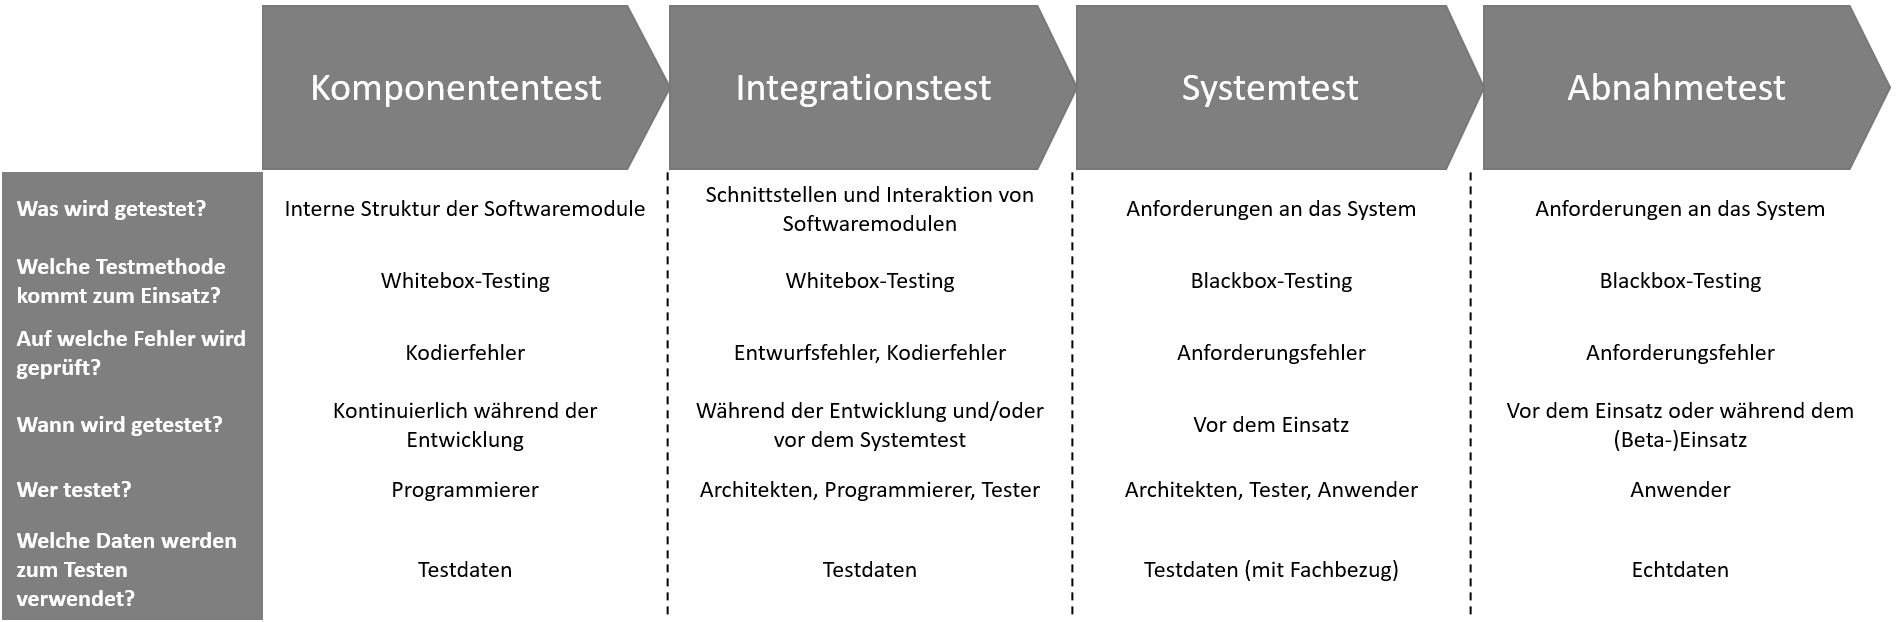
\includegraphics[width=1.05\textwidth]{teststufen.png}
\end{figure}
\scriptsize{Quelle: \href{https://upload.wikimedia.org/wikipedia/commons/9/9c/Eigenschaften_der_Teststufen_II.png}{\url{https://upload.wikimedia.org/wikipedia/commons/9/9c/Eigenschaften_der_Teststufen_II.png}}}
\end{frame}

\section{Literaturverzeichnis}

\frame{
\frametitle{Literaturverzeichnis}
\begin{thebibliography}{10}
  \bibitem{ATB} Austrian Testing Board, German Testing Board e. V. \& Swiss Testing Board: \emph{ISTQB Certified Tester -- Lehrplan Foundation Level}. Version 4.0.1a, \href{https://www.austriantestingboard.at/wp-content/uploads/2023/09/ISTQB_CTFL_Lehrplan-2023_V4.0.1a_DE.pdf}{\url{https://www.austriantestingboard.at/wp-content/uploads/2023/09/ISTQB_CTFL_Lehrplan-2023_V4.0.1a_DE.pdf}}, 16. August 2023
  \bibitem{GTB} German Testing Board e. V.: \emph{ISTQB Certified Tester --  	Lehrplan Advanced Level Technical Test Analyst}. Version 4.0 DE, \href{https://www.gtb.de/wp-content/uploads/2023/10/CTAL-TTA_v4.0_DE_-Advanced-Syllabus-1.pdf}{\url{https://www.gtb.de/wp-content/uploads/2023/10/CTAL-TTA_v4.0_DE_-Advanced-Syllabus-1.pdf}}, 5. Januar 2022
\end{thebibliography} 
}

\frame{
\frametitle{Literaturverzeichnis}
\begin{thebibliography}{10}
  \bibitem{GLO} ISTQB: \emph{Glossar}, \href{https://glossary.istqb.org/de_DE/}{\url{https://glossary.istqb.org/de_DE/}}, 16. Oktober 2024
  \bibitem{MSCH} Maud Schlich: \emph{Softwaretesten nach ISTQB CTFL 4.0 für Dummies}, 1. Auflage 2024, Wiley-VCH GmbH
\end{thebibliography} 
}

\end{document}